\section{Signale}
\label{sec:signale}

\begin{frame}{Frequenzen}
    \begin{columns}
        \begin{column}{0.5\textwidth}
            \centering{Verteilung der Frequenzen}
            \begin{table}
                \centering
                \begin{tabular}{c S[table-format=1.0]}
                    \toprule
                    {Satellit} & {\# Frequenzen} \\
                    \midrule
                    Block IIA   & 1 \\
                    Block IIR   & 2 \\
                    Block IIR-M & 3 \\
                    Block IIF   & 4 \\
                    GPS III     & 5 \\
                    GPS IIIF    & 5 \\
                    \bottomrule
                \end{tabular}
            \end{table}
        \end{column}
        \begin{column}{0.5\textwidth}
            \centering{Namen der Frequenzen}
            \begin{table}
                \centering
                \begin{tabular}{c S[table-format=4.2]}
                    \toprule
                    {Name} & {$f\:/\:\si{\mega\hertz}$} \\
                    \midrule
                    L1 C/A  & $\num{1575.42}$ \\
                    L1 P(Y) & $\num{1575.42}$ \\
                    L2C     & $\num{1227.60}$ \\
                    L5      & $\num{1176.45}$ \\
                    L1C     & $\num{1575.42}$ \\
                    \bottomrule
                \end{tabular}
            \end{table}
        \end{column}
    \end{columns}
\end{frame}

\begin{frame}{Das Signal}
    \begin{columns}
        \begin{column}{0.5\textwidth}
            Informationen im Signal
            \begin{itemize}
                \item Satellitenposition
                \item Zeit
                \item Uhrzeitkorrekturen
                \item Systeminformationen
                \end{itemize}\pause
        \end{column}
        \begin{column}{0.5\textwidth}
            \begin{figure}
                \centering
                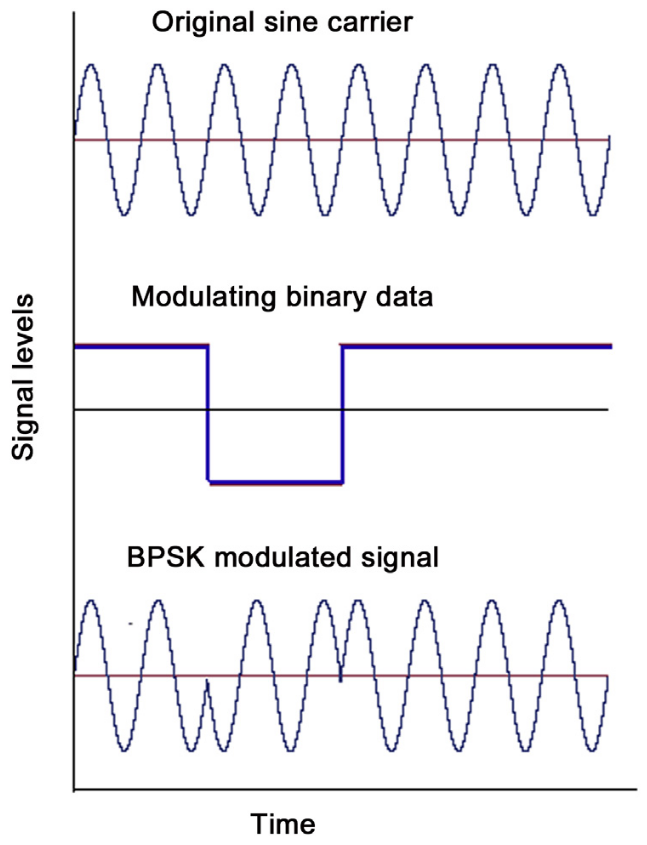
\includegraphics[width=0.6\textwidth]{images/signalzusammensetzung.png}
            \end{figure}
            Wellenzusammensetzung {\small[Acharya]}
        \end{column}
    \end{columns}
\end{frame}
